\documentclass[12pt]{report}
\usepackage[utf8]{inputenc}

% TODOs in the document
\setlength{\marginparwidth}{2cm}
\usepackage{todonotes}%TODOs
\usepackage{float}
\usepackage{graphicx}% Images
\graphicspath{ {images/} }
\usepackage{amsmath}% Math
\usepackage{titlesec}
\titleformat{\chapter}{\normalfont\huge\bfseries}{\thechapter}{1em}{}
\usepackage[a4paper, width=150mm, top=25mm, bottom=25mm, bindingoffset=6mm]{geometry}% Page layout
\usepackage[backend=biber, style=apa, citestyle=apa]{biblatex}% Configured "biblatex" package with "Biber" backend
\addbibresource{references.bib}% Bibliography file
\usepackage{hyperref}% Hyperlinks
\hypersetup{
    colorlinks=true,
    linkcolor=black,
    citecolor=black,
    filecolor=magenta,      
    urlcolor=cyan,
}
\usepackage{ragged2e}% Justify text
\usepackage[justification=justified]{caption}% Caption justification
\usepackage[labelfont=bf]{caption}
\usepackage[labelfont=it,textfont={it},justification=centering]{subcaption}
\usepackage{listings}
\lstset{
    basicstyle=\ttfamily, % Set the basic style for code to typewriter font
    breaklines=true,       % Allows automatic line breaking
    breakatwhitespace=false, % Allows breaking lines at whitespace
}
\usepackage{adjustbox}%fit table to page
\newcommand{\CellWithForcedBreak}[2][c]{% #1 = alignment, #2 = contents
    \begin{tabular}[#1]{@{}c@{}}#2\end{tabular}}

\usepackage{tikz}% Background color

\begin{document}

\begin{titlepage}
    \centering
    \vspace*{1cm}
    \makebox[\textwidth][c]{\Huge\bfseries Epileptic Neural Dynamics:}\\
    \makebox[\textwidth][c]{\Huge\bfseries Insights from a Computational Model}\\
    \makebox[\textwidth][c]{\Huge\bfseries of a CA3 Hippocampal Network}\\[1cm]
    \Large by\\[1cm]
    \Large \textbf{Marc Julius Posthuma}\\[1cm]
    \Large Radboud University, in affiliation with Synaptica B.V.\\[2cm]

    % Images side by side
    \noindent
    \begin{minipage}[c]{0.5\textwidth}
        \centering
        \includegraphics[height=3cm,keepaspectratio]{Radboud_Universiteit_Nijmegen-logo.png}
    \end{minipage}%
    \begin{minipage}[c]{0.5\textwidth}
        \centering
        \includegraphics[height=1cm,keepaspectratio]{synaptica_logo.png}
    \end{minipage}

    \vspace{1cm} % Adjust vertical space as needed

    % Text blocks side by side
    \noindent
    \begin{minipage}[t]{0.5\textwidth}
        \centering
        \Large Readers:\\
        1st: Prof.\ Dr.\ P.H.E. Tiesinga\\
        2nd: Prof.\ Dr.\ R.J.A. van Wezel
    \end{minipage}%
    \begin{minipage}[t]{0.5\textwidth}
        \centering
        \Large Supervised by:\\
        Dr.\ Marijn Martens (CEO)\\
        Sean Gies, MSc
    \end{minipage}

    \vfill

    \footnotesize Thesis submitted in partial fulfillment of the requirements
    for the degree of Master of Science in Medical Biology (Specialization: Neurobiology)\\[1cm]
    \Large April 26th, 2024
\end{titlepage}

\listoftodos% Remove this line when you're done with the document

\addcontentsline{toc}{chapter}{Copyright Statement}
\section*{Copyright Notice}
Contents of this thesis, including data and software, were produced and/or utilized
under a signed agreement with Synaptica B.V., and are considered proprietary.

\subsection*{Data and Code Availability}
The datasets and computer code utilized in the simulations and subsequent analyses within this thesis
are proprietary assets owned by Synaptica B.V. Software includes the ``Neuromics'' and ``Network\_Sims'' packages
developed by Synaptica B.V. These materials are not available to the public,
and all rights to their use are exclusively reserved by Synaptica B.V.
Inquiries regarding access to the data and code for replicating experiments or for further analysis of
the results should be directed to Synaptica B.V., attention Marijn Martens.
% End the current paragraph and add space
\par
\vspace{12pt} % You can adjust the space to more or less as per your need

% Start a new un-indented line for the email
\noindent Requests can be sent via email to \textbf{\textcolor{blue}{\texttt{info@synaptica.nl}}}.

\vspace{12pt}

\begin{figure}[h]
    \centering
    \includegraphics[height=1cm,keepaspectratio]{synaptica_logo.png}
\end{figure}

\vfill

\subsection*{Declaration of Originality}
I hereby declare that this thesis, titled \textit{``Epileptic Neural Dynamics: Insights from a Computational
    Model of a CA3 Hippocampal Network''}, is my own original work and has been written by me.
All sources and materials used have been properly acknowledged and referenced.
This thesis has been prepared in accordance with the rules and regulations set by the exam committee of the FNWI,
Radboud University, regarding plagiarism. I affirm that this work has not been submitted for any other
academic degree or professional qualification.\\

\noindent Marc Julius Posthuma\\
26th of April, 2024

\begin{figure}[h]
    \centering
    \includegraphics[height=2cm,keepaspectratio]{Radboud_Universiteit_Nijmegen-logo.png}
\end{figure}
\addcontentsline{toc}{chapter}{Abstract}
\section*{Abstract}
Temporal lobe epilepsy (TLE) is a frequently occurring form of epilepsy, commonly
associated with the hippocampus, particularly its CA3 subfield, which is noted
for its hyperexcitability and crucial role in seizure generation. This study
employs a computational model of the CA3 subfield, developed within the NEURON
simulation environment, comprising 800 pyramidal cells, 200 basket cells, and 200
oriens-lacunosum moleculare (OLM) interneurons. To simulate genetic profiles
characteristic of epilepsy, network alterations were introduced to sodium and
potassium conductances across all cell types. The study examines the impact of
these alterations on neural oscillations within the theta-gamma frequency range
and their power. Additionally, it investigates the network's susceptibility to
depolarization blocks in basket cell populations resulting from increased external
noise. An in-depth exploration of population burst dynamics was also conducted.
Furthermore, the effects of strengthened recurrent connections in the basket cell
population were examined to assess the potential for rescuing the network from an
ictal state back to homeostatic baseline activity. The findings suggest that the
CA3 network is indeed hyperexcitable, with imbalances in sodium and potassium
channels that mirror genetic predispositions for epilepsy, leading to increased
firing rates and heightened susceptibility to epileptiform activity. Moreover, the
network demonstrated increased resilience to depolarization blocks through enhanced
soma-inhibition by recurrently connected basket cells, showing effects akin to
those of contemporary anti-epileptic drugs (AEDs) and other therapeutic interventions.

\textbf{Keywords:} Temporal lobe epilepsy; CA3; hippocampus; computational neuroscience; NEURON\@;
depolarization block; ictal state; oscillations
\addcontentsline{toc}{chapter}{Acknowledgements}
\section*{Acknowledgements}
I am immensely grateful to Marijn Martens and Sean Gies for their guidance and
mentorship during my six-month internship at Synaptica B.V. Their expertise
was crucial in both practical and theoretical aspects of my work as a
Master's student.
Marijn Martens provided invaluable insights that enhanced my analytical thinking
and problem-solving skills, vital for completing this thesis. The opportunity to
work at Synaptica B.V., with access to excellent computational resources and
travel support, greatly contributed to my experience.
Observing the company's growth and the scale of projects managed by Sean,
Arthogrul, and their teams was particularly inspiring. It was motivating to see
the progress made over my tenure, adding a valuable perspective to my career
path.
Special thanks to Sean Gies for his thorough and patient explanations of complex
technical processes, which deepened my understanding of programming significantly.
Both Marijn and Sean were always approachable, providing feedback and fostering
a collaborative environment that supported my development as a researcher.
I am also thankful to the entire team and fellow students at Synaptica B.V. for
their support and encouragement throughout my internship. Their feedback
and suggestions played a significant role in shaping my research direction.
This thesis has undoubtedly benefited from their profound professional guidance,
and for that, I am truly thankful.
\pagestyle{empty} % Disable page numbers

% Full page background color
\begin{tikzpicture}[remember picture,overlay]
    \fill[black!20] (current page.south west) rectangle (current page.north east);
\end{tikzpicture}

\vspace*{\fill}
\begin{center}
    \begin{minipage}{.8\textwidth}
        \centering
        \textit{``Every man can, if he so desires, become the sculptor of his own brain''}
        \vspace{10pt}
        \textbf{--- Santiago Ramón y Cajal}
    \end{minipage}
\end{center}
\vspace*{\fill}

\tableofcontents
\listoffigures
\listoftables
% Include your chapters
\chapter{Introduction}

\todo[inline, color=red!40]{This chapter is the current work in progress.}
\todo[inline, color=red!40]{see the introduction-outline.md file to see what to do for this chapter.}
\todo[inline]{ADD REFERENCES TO THE TEXT}

\section{Background}
In this chapter, the research topic is introduced. 
The chapter starts with a brief overview of epilepsy, followed by a discussion on the role of the hippocampus in temporal lobe epilepsy. 
The chapter then discusses the role of the CA3 region of the hippocampus in epilepsy. 
The chapter then discusses the role of computational modeling in neuroscience. 
Finally, the chapter discusses the literature gap that this research aims to address.

\subsection{Introduction to Epilepsy and Its Complexity}
Epilepsy is a neurological disorder characterized recurrent seizures. 
Seizures have to be two or more unprovoked and more than 24 hours apart, a single unprovoked
seizure with a high recurrence risk (>60 \% over the next 10 years); or the patient needs to have been previously diagnosed with an epilepsy syndrome.
Patients with epilepsy usually also suffer cognitive challenges, language difficulties, and an increased risk of mental health issues, 
such as anxiety and depression~\parencite{fisherILAEOfficialReport2014}. At its core, epilepsy 
involves an imbalance between excitatory and inhibitory processes within the brain. 
This imbalance can originate in specific brain regions and spread, affecting various interconnected areas 
outside of the epileptogenic zone~\parencite{ludersEpileptogenicZoneGeneral2006}.
The minimum amount of brain tissue of an associated region that initiates a seizure is therefore not fixed and is the 
reason epilepsy is often though of as a network disorder.

\subsection{Temporal Lobe Epilepsy: A Closer Look}
Temporal Lobe Epilepsy (TLE), the most prevalent form of focal epilepsy in adults, 
impacts over 50 million people globally. TLE's epileptic events often begin in 
brain regions like the hippocampus and entorhinal cortex, known for their 
capacity to independently produce epileptiform activities~\parencite{lyttonComputerSimulationEpilepsy2005}.
Despite many TLE patients not responding to medication, research into TLE's 
underlying mechanisms is vital for developing new treatments.

\subsection{The Hippocampus and Its Role in TLE}
The hippocampus, located in the temporal lobe, is crucial for memory formation 
and retrieval, emotion regulation, and spatial navigation. In TLE, it often 
serves as the seizure's focal point, especially its CA3 subfield. The CA3 region, 
with its dense connections and low epilepsy activation threshold, is particularly 
susceptible to hyper-excitability~\parencite{witterIntrinsicExtrinsicWiring2007}. Seizures can be 
triggered by excessive stimulation from the entorhinal cortex, highlighting the 
complex interplay between different brain regions in TLE\@.

\subsection{Functional Brain Networks in Epilepsy}


\subsection{Neural Oscillations and Epilepsy}
Characteristic neural oscillations in the hippocampus, such as theta (3--12 Hz) 
and gamma (30--80 Hz) rhythms, play significant roles in memory and cognition. 
Epilepsy is associated with alterations in Cross-Frequency Coupling (CFC), where 
the phase of slower waves modulates the amplitude of faster waves, reflecting 
disrupted network functionality. Abnormalities in Theta-Gamma Phase-Amplitude 
Coupling (PAC) correlate with cognitive impairments in epilepsy, underscoring 
the importance of understanding these oscillations in neurological disorders.

\subsection{Interictal Network Dynamics}
The interictal state, marking intervals between seizures, reveals sporadic 
spiking in local field potentials (LFPs) indicative of abnormal electrical 
activity. These intermittent bursts highlight the underlying dysfunction in 
neural processing characteristic of epileptic networks, even outside of 
seizure episodes.

\subsection{Sodium and Potassium Channels in Epilepsy}
Sodium and potassium channels are essential for maintaining the resting
membrane potential and action potential generation in neurons.
Dysfunctional sodium and potassium channels can lead to hyperexcitability in neurons.
\subsection{Computational Modeling in Neuroscience with NEURON}
The NEURON simulator is a powerful tool for modeling the intricate dynamics 
of neurons and their networks. It supports detailed simulations of membrane 
dynamics, synaptic interactions, and the Hodgkin-Huxley model for action 
potentials. NEURON's Python interface facilitates scripting and integration 
with other Python-based tools, enhancing its utility in neuroscience research.
This simulator is crucial for studying neural phenomena, the effects of 
anti-epileptic drugs, and diseases caused by dysfunctional ion channels, 
providing invaluable insights into the functioning of the nervous system 
and the development of therapeutic strategies.

\subsection{Aim of the research}
This study aims to further investigate the role of the CA3 region of the hippocampus in epilepsy, 
by adapting the computational model of the CA3 region of the hippocampus by~\textcite{neymotinKetamineDisruptsTheta2011} in the NEURON simulator.
The model consists of 800 pyramidal, 200 O-LM interneurons and 200 basket cells. 
The baseline model contains enough biophysical detail to replicate homeostatic neural activity, consisting of theta-modulated gamma oscillations.

This research builds upon experiments by~\textcite{sanjayImpairedDendriticInhibition2015}, 
which focussed on reducing dendritic inhibition, increasing external stimulation and modifying synaptic connectivity as potential causes for TLE\@.

Instead, this study will focus on the role of sodium and potassium channels via ion-conductance modifications throughout the network, 
the sensitivity for external noise in such conditions and the effects varied recurrent connectivity.

\subsection{Literature Gap}

\section{Research question}

\section{Outline of the thesis}
\chapter{Methods}
This chapter describes the methods used in this research.\todo[inline,
    color=red!40]{check the text in the computer settings used in simulations}% New todo added here

\section{Computational model}
\textit{Description of the model implementation.}

The network model that was used in this research is a custom implementation
made by \textcite{sanjayImpairedDendriticInhibition2015}. This model is based
on the CA3 subfield region of the hippocampus and is implemented in the NEURON
simulation environment using python version 3.9.16 as an interface
\href{https://www.neuron.yale.edu}{(\url{https://www.neuron.yale.edu)}}. The
model consists of 1000 neurons, which are divided into populations of 800
pyramidal cells and 200 soma-inhibiting basket cells and 200 Oriens-Lacunosum
Moleculare (O-LM) interneurons. The implementation used in this research made
in cooperation with Sean Gies is part of the \textit{Neuromics} software
package by Synaptica Ltd.

\begin{figure}[htbp]
    \centering
    \includegraphics[width=0.5\textwidth]{model_design.png}
    \caption[Schematic of the CA3 network model]{Schematic of the CA3 network model.}
    \begin{minipage}{0.9\textwidth}
        The network comprises of many microcircuits with the connectivity as shown in the above figure. Pyr cells (pyramidal), BC cells (basket cells that inhibit soma),
        OLM cells (oriens lacunosum moleculare interneurons that inhibit dendrites), external inputs (mainly from the entorhinal cortex) to Pyr cells, and MS (medial septum).
        BC and OLM cells are stimulated by Pyr cells, while Pyr cells are inhibited by BC and OLM cells.
        Recurrent connections among Pyr cells are excitatory, whereas those among BC cells are inhibitory.
        OLM cells are inhibited by BC cells. The medial septum (MS) delivers inhibitory inputs every 150 ms to BC and OLM cells.
    \end{minipage}\label{fig:model_design}
\end{figure}\pagebreak

This is a test reference to figure~\ref{fig:model_design}, see it works!%remove later

\section{Model implementation: cell parameters}
The model consists of three types of neurons, each with its own set of
parameters and defined cell classes. The parameters for each cell type are
based on the following references:
\begin{enumerate}
    \item \textbf{Basket Cells}: Modeled after \textcite{wangGammaOscillationSynaptic1996},
          featuring standard dynamics for Na and K currents, along with synaptic and leak currents.
          Each cell is modeled as a single compartment and obeys the following current balance equation:
          \begin{equation}
              C_I \frac{dV_I}{dt} = I_{\text{app},I} - I_{\text{Na},I} - I_{\text{K},I} - I_{\text{L},I} - I_{\text{syn},I}
          \end{equation}

          where \(V_I\) is the membrane potential (mV), \(C_I = 1 \, \mu\text{F/cm}^2\)
          is the membrane capacitance, \(I_{\text{app},I}\) is the applied current, and
          \(I_{\text{syn},I}\) is the total synaptic current. The leak current
          \(I_{\text{L},I} = g_{\text{L},I}(V_I - E_{\text{L},I})\) has a conductance
          \(g_{\text{L},I} = 0.1 \, \text{mS/cm}^2\) and reversal potential
          \(E_{\text{L},I} = -65 \, \text{mV}\). All currents are in units of
          \(\mu\text{A/cm}^2\). The sodium \(I_{\text{Na},I}\) and potassium
          \(I_{\text{K},I}\) currents are voltage-dependent spiking currents of the
          Hodgkin-Huxley type.
    \item \textbf{O-LM Cells}: Adapted from \textcite{saragaActiveDendritesSpike2003},
          including additional currents like hyperpolarization-activated (h) and A-type currents.
          Each cell is modeled as a single compartment and obeys the following current balance equation:
          \begin{equation}
              C_O \frac{dV_O}{dt} = I_{\text{app},O} - I_{\text{Na},O} - I_{\text{K},O} - I_{\text{L},O} - I_{\text{h},O} - I_{\text{A},O} - I_{\text{syn},O}
          \end{equation}

          where \(V_O\) is the membrane potential, \(C_O = 1.3 \, \mu\text{F/cm}^2\) is
          the membrane capacitance, \(I_{\text{app},O}\) is the applied current, and
          \(I_{\text{syn},O}\) is the total synaptic current. The leak current
          \(I_{\text{L},O} = g_{\text{L},O}(V_O - E_{\text{L},O})\) with conductance
          \(g_{\text{L},O} = 0.05 \, \text{mS/cm}^2\) and reversal potential
          \(E_{\text{L},O} = -70 \, \text{mV}\). \(I_{\text{Na},O}\), \(I_{\text{K},O}\),
          \(I_{\text{h},O}\), and \(I_{\text{A},O}\) represent the transient sodium,
          delayed rectifier potassium, hyperpolarization-activated (or h) mixed-cation,
          and A-type potassium currents, respectively, all in units of
          \(\mu\text{A/cm}^2\).
    \item \textbf{Pyramidal Cells}: Based on \textcite{miglioreDendriticIhSelectivelyBlocks2004},
          incorporating compartmentalized dynamics for the complex morphology of pyramidal neurons.
          Each cell is modeled as a multi-compartmental neuron with 5 compartments: 1 for basal dendrites (Bdend),
          1 for soma, and 3 for apical dendrites (Adend1, 2 and 3). Each compartment obeys the following current balance equation:
          \begin{equation}
              C_{E_k} \frac{dV_{E_k}}{dt} = I_{\text{app},E_k} - I_{\text{Na},E_k} - I_{\text{K},E_k} - I_{\text{L},E_k} - I_{\text{h},E_k} - I_{\text{A},E_k} - I_{\text{syn},E_k} + I_{\text{conn},E_k}
          \end{equation}

          where \(V_{E_k}\) is the membrane potential of compartment \(k\), \(C_{E_k}\)
          is the membrane capacitance, \(I_{\text{app},E_k}\) is the applied current,
          \(I_{\text{syn},E_k}\) is the total synaptic current, and
          \(I_{\text{conn},E_k}\) represents the current due to electrical coupling
          between compartments. \(I_{\text{L},E_k}\), \(I_{\text{Na},E_k}\),
          \(I_{\text{K},E_k}\), \(I_{\text{h},E_k}\), and \(I_{\text{A},E_k}\) denote the
          leak, transient sodium, delayed rectifier potassium,
          hyperpolarization-activated mixed-cation, and A-type potassium currents for
          compartment \(k\), respectively.

\end{enumerate}
\pagebreak

\section{Model implementation: synaptic connections}
The model contained three types of synaptic connections: excitatory, inhibitory
based on AMPA, NMDA and GABA-A receptors. Synapses were modeled by standard
NEURON double-exponential mechanism. The synaptic connections were implemented
as follows:

\begin{table}[htbp]
    \centering
    \caption[Synaptic Parameters for the Connectivity Between Neurons in the Model]{Synaptic Parameters for the Connectivity Between Neurons in the Model: Pre- and postsynaptic receptor types are given for each cell type.
        The time constants \(\tau_1\) and \(\tau_2\) are in milliseconds.
        \(\tau_1\) is the rise time constant, the time it takes for synaptic conductance to increase from baseline to peak.
        \(\tau_2\) is the decay time constant, the time it takes for the conductance to decrease from peak to baseline.
        The conductance indicates the strength of the synaptic connection and its ability to conduct ionic current across the postsynaptic membrane.
        This influences the extent to which the synaptic input can depolarize the postsynaptic neuron and is in nanoSiemens (nS).}
    \begin{tabular}{lllccc}
        \hline
        Presynaptic & Postsynaptic & Receptor & \(\tau_1\) (ms) & \(\tau_2\) (ms) & Conductance (nS) \\
        \hline
        Pyramidal   & Pyramidal    & AMPA     & 0.05            & 5.3             & 0.02             \\
        Pyramidal   & Pyramidal    & NMDA     & 15              & 150             & 0.004            \\
        Pyramidal   & Basket       & AMPA     & 0.05            & 5.3             & 0.36             \\
        Pyramidal   & Basket       & NMDA     & 15              & 150             & 1.38             \\
        Pyramidal   & OLM          & AMPA     & 0.05            & 5.3             & 0.36             \\
        Pyramidal   & OLM          & NMDA     & 15              & 150             & 0.72             \\
        Basket      & Pyramidal    & GABA-A   & 0.07            & 9.1             & 0.72             \\
        Basket      & Basket       & GABA-A   & 0.07            & 9.1             & 4.5              \\
        Basket      & OLM          & GABA-A   & 0.07            & 9.1             & 0.0288           \\
        OLM         & Pyramidal    & GABA-A   & 0.2             & 20              & 72               \\
        MS          & Basket       & GABA-A   & 20              & 40              & 1.6              \\
        MS          & OLM          & GABA-A   & 20              & 40              & 1.6              \\
        \hline
    \end{tabular}\label{tab:synaptic_parameters}
\end{table}

\section{Model implementation: stimulation and noise}
\todo[inline,
    color=red!40]{Netstim information is missing.}% New todo added here

The model was activated by external inputs originating from the entorhinal
cortex, which were then transmitted to the pyramidal cells. Background random
excitatory and inhibitory inputs were received by the OLM, basket cells, and
the soma of the pyramidal cells via their AMPA, NMDA, and GABA-A receptors as
shown in table~\ref{tab:synaptic_parameters}. Similarly, the distal dendritic
compartments of the pyramidal cells also received comparable inputs through the
same types of receptors. Connections such as OLM to pyramidal cell, basket to
pyramidal cell, basket-basket recurrent connections, and medial septum to OLM
and basket cell connections were mediated through GABA-A receptors.
Additionally, the medial septum provided inhibitory inputs to the basket and
OLM cells at intervals of 150 ms.

\section{Simulations}
For the simulations, the model was implemented in NEURON version 7.6.3. The
simulations were run on a Linux GNOME (v22.04) desktop computer with an Intel
Core i7--8700K processor with 60 cores for multithreading, a Nvidia GTX 4060
graphics card, and 32 GB of RAM\@. Trials were run for 5000 ms with a time
integration step of 0.1 ms resulting in 50.000 simulation steps per trial
dataset. Random seeds were used to generate the external noise, connections and
cells for each trial and remained constant between trials and between
experiments. The number of trials varies between experiments and are specified
in their respective sub-sections that follow. In the network, the individual
cells are assigned a global identifier to which all the data is associated in
the same ascending order for each trial. The first 800 cells were always
pyramidal cells, the next 200 were basket cells and the last 200 were OLM
cells. For each trial, the individual cell spike times are saved for the entire
duration of the simulation. Pyramidal cell membrane soma voltage data was saved
per cell in order to calculate the LFP signal (necessary for theta-gamma
calculations).

\subsection{Baseline activity}
In order to obtain baseline activity in the network as shown in figure
~\ref{fig:model_design}, current injections were added (\textbf{Pyramidal
    cells:} 50 pA\@; \textbf{OLM cells:} -25 pA). At Baseline, the network
generates theta-modulated gamma oscillations activity. This activity was
measured from the Local Field potential (LFP) in the network. The LFP was
simulated by a sum difference between membrane potential of the distal apical
and basal dendritic compartment over all pyramidal cells. As discussed in the
cell parameters section, all cells contained leak current, transient sodium
current \(I_{\text{Na}}\), and delayed rectifier current \(I_{K, \text{-}
        \text{dr}}\) to allow for action potential generation. On average, the firing
rates were \(2.36 \pm 0.024\) Hz for pyramidal cells, \(16.05 \pm 0.15\) Hz for
basket cells and \(0.96 \pm 0.027\) Hz for O-LM interneurons at baseline in the
original \parencite{sanjayImpairedDendriticInhibition2015}. However, it should
be noted that our custom implementation of the same model had a slightly
lowered baseline (see the results section). The reason for this discrepancy is
unknown and is a potential source of error in the results. 50 trials total were
done for the baseline activity and averaged.

\subsection{Model validation}
In order to test the implementation of the model, results from the article were
replicated, namely figures 6A, B and C from
\textcite{sanjayImpairedDendriticInhibition2015}. In this replicated experiment
the OLM to pyramidal cells connection weight was reduced in decrements of 0.1x
times the baseline from 1.0 to 0.0. In addition to reduced connection strength,
the external noise fed into the pyramidal cells was increased in increments of
0.1X times the baseline from 1.0 to 2.0. By reducing the connectivity from OLM
to pyramidal cells, dendritic inhibition was impaired and potential
epileptiform activity was induced. The original results on which the validation
experiment focussed on, were the following three aspects: changes in firing
rates per population, the changes in dominant theta and gamma frequencies, and
finally the changes in the power of the theta and gamma oscillations.

\subsection{Sodium and potassium variants}
In this experiment, the sodium and potassium conductances of the all cell types
cells were changed from 0.5x to 1.5x times the baseline in increments of 0.1.
The changes were induced in separate experiments for each of the three cell
types, so 6 experiments in total were conducted: 3 for sodium and 3 for
potassium. These induced changes were done in order to investigate the effect
of the conductances on the network activity and the influence of individual
cell types on the same metrics as in the model validation experiment. 20 trials
each were done per condition (6 total conditions) and the results were
averaged.

\subsection{External noise variants}
In this experiment, the external noise fed into the pyramidal cells was set a
new baseline for the 1.0x condition, which was 20 times that of the original
\textcite{sanjayImpairedDendriticInhibition2015} model. Reduced OLM to pyr
connections were kept at 10\% of the original baseline. This was done because
in the original article, epileptic activity was induced by feeding in 20 times
more external noise at reduced dendritic inhibition. This condition was tested
as a special condition in figure 7 of the article, and was expanded upon
because of the occurrence of a depolarization block in the basket cell spike
activity. This depolarization block occurrence was assumed to be the epileptic
state in which the network is found at such conditions. This new baseline was
changed times a range of pyramidal noise factors of the following values: 0.65,
0.70, 0.75, 0.80, 0.85, 0.90, 0.95, 1.00, 1.10, 1.20, and 1.30. In addition to
the range of noise factors, pyramidal conductances \(g_{\text{Na}}\) and
\(g_{\text{K}}\) were modified over a range of 0.5x to 1.5x times the baseline
in increments of 0.1. 15 trials were done per noise condition and the results
were averaged.

\subsection{Recurrent connection strength variants}
In this experiment, the recurrent connection strength between basket cells was
modified over the following range: 1.00, 1.05, 1.10, 1.15 and 1.20 times the
baseline. This was done in order to investigate the possibility of rescuing the
epileptic network back to baseline activity by increased the strength of soma
inhibition. Similarly to the external noise variants, \(g_{\text{Na}}\) and
\(g_{\text{K}}\) were modified over a slightly tighter range of plus or minus
25\% of the baseline and including baseline of 1.00. Again, the OLM to
pyramidal connection weight was kept at 10\% in order to be able to evoke the
depolarization block in basket cell spike activity, while also feeding the 20x
external noise to the pyramidal cells. 15 trials were done per condition and
the results were averaged. 15 trials were done per condition and the results
were averaged.

\todo[inline,
    color=red!40]{check the methodology for convolutions and depolarization blocks. Remove excess text at DPB explanation}% New todo added here

\subsubsection{Detection of epileptiform activity (Experiment: External noise variants)}
The detection of epileptic activity depends on the spiking activity of the
basket cells, which from figure 7 from the
\textcite{sanjayImpairedDendriticInhibition2015} article occurs in the presence
of great external drive from the pyramidal cells of at least 20 times the
baseline and with reduced dendritic inhibition by the OLM cells. Detection of a
depolarization block in the basket cells was done by calculating the convoluted
fire rates of the basket cell population.

\noindent The systematic approach to analyzing basket cell firing rates through
convolution with a Gaussian window was as follows:
\begin{itemize}
    \item \textbf{Extracting Spike Times:} The \lstinline{get_spike_times_for_basket_cells}
          function is used for iterating over a range of GIDs. This process collects spike times from
          all basket cells and concatenates them, constructing a continuous signal of neural activity.

    \item \textbf{Creating Time Series:} Spike times are converted into a binary series
          using \lstinline{create_time_series}. Each neural firing event is denoted by a '1' in a
          zero-initialized array at the corresponding time index.

    \item \textbf{Applying Gaussian Convolution:} The \lstinline{apply_gaussian_convolution}\newline
          function smooths the time series. It convolves the series with a Gaussian window, normalized
          to sum to one, yielding a signal that mirrors the firing rates over time.

    \item \textbf{Summing Convolved Signals:} Collective firing behavior is analyzed by
          \lstinline{get_convolved_signal_per_neuron}. It applies Gaussian convolution to individual
          neuron time series and sums them, forming an aggregated firing rate signal.

    \item \textbf{Detecting Depolarization Blocks:} The \lstinline{detect_depolarization_blocks}
          function identifies reduced activity periods by analyzing the convolved signal for intervals
          that remain below a set threshold for a specified minimum duration.
\end{itemize}

\noindent For detecting depolarization blocks in the basket cell population, the
methodology was as follows:
\begin{itemize}
    \item Establishing a signal threshold indicating a depolarization block.
    \item Excluding initial transient analysis to prevent false positives.
    \item Identifying threshold crossings that mark the start and end of depolarization
          blocks.
    \item Applying a minimum duration filter to these blocks.
    \item Summarizing and reporting the total duration of all valid depolarization blocks
          in the trial.
\end{itemize}

\noindent A check was performed if the convoluted signal remained beneath a fixed
threshold of 0.001 for at least 100 ms. This threshold was defined non-zero,
yet tiny as in the depolarization block there are no firing neurons in the
basket population. The first 50 ms of the signal were excluded to avoid false
positives. If the signal remained beneath the threshold for at least 100 ms,
the condition was considered to be in a depolarization block state. This was
done for each trial individually.\pagebreak

\subsubsection{Detection of epileptiform activity (Experiment: Recurrent connection strength variants)}

\subsubsection{Burst detection around depolarization blocks}
\chapter{Results}

\todo[inline]{fix the captions for the figures, see the article for the correct captions.}

\section{Results of the Baseline activity}
In the initial experiment, the baseline activity of the CA3 network was
observed from the \textit{original model} by
\textcite{sanjayImpairedDendriticInhibition2015}. The network was simulated for
5000 ms and showed somewhat synchronous activity throughout all three
populations (pyr, BC and OLM). Basket cells showed a higher firing rate
compared to the pyramidal cells and OLM cells. The basket cells seem to swap
between states of synchrony and asynchrony which is not observed in the other
two populations. The OLM cells showed a lower firing rate compared to the
pyramidal cells and basket cells. The baseline activity of the CA3 network is
shown in figure~\ref{fig:baseline_activity}.

\begin{figure}[htbp]
    \centering
    \includegraphics[width=0.9\textwidth]{Network_spike_activity_OLM_baseline.png}
    \caption[Baseline activity of the CA3 network]{Baseline activity of the CA3 network.}\label{fig:baseline_activity}
    \begin{minipage}{0.9\textwidth}
        The above figure shows the baseline activity of the CA3 network. The network was simulated for 5000 ms. The spike activity in time of the Pyr cells, BC cells, and OLM cells are shown based on the Neuron ID\@. ID 0--799 = Pyramidal (blue), 800--999 = BC (green), 1000--1200 = OLM (red). The x-axis represents the time in ms and the y-axis represents the neuron ID\@.
    \end{minipage}
\end{figure}

\section{Results of the Model validation}
To test whether our implementation of the CA3 network was able to replicate
more elaborate results, results from figure 6 of the original
\textcite{sanjayImpairedDendriticInhibition2015} article were replicated in
figure~\ref{fig:validation_firing_rates},~\ref{fig:validation_frequencies} and
~\ref{fig:validation_power}. The results show that the model was able to
replicate the results of the original article with slightly lower firing rates,
theta-gamma frequencies and power, which can be seen in
table~\ref{tab:validation_results}. The original article results are visible in
the methods section in table~\ref{tab:original_validation_results}.

\begin{figure}[htbp]
    \centering
    \includegraphics[width=0.9\textwidth]{Sanjay_validation_firing_rates.png}
    \caption[Validation of the firing rates]{Validation of the firing rates.}\label{fig:validation_firing_rates}
    \begin{minipage}{0.9\textwidth}
        The above figure shows the firing rates of the Pyr cells, BC cells, and OLM cells when dendritic inhibition is decreased and external noise is increased.
        The firing rates were calculated from the spike activity of the cells in each population for the duration of the simulation (5000 ms).
        The double x-axis represents both decrement in the weight of dendritic inhibition on pyramidal cells by OLM interneurons,
        while simultaneously increasing external noise stimulation to pyramidal cells.
        External noise levels rise and inhibition decreases by increments of 0.1, each representing a 10\% change relative to the baseline.
        The y-axis represents the firing rate in Hz.
        The firing rates are per cell type: Pyr (blue), Basket (green) and OLM (red).
        The error bars represent the standard deviation of the firing rates.
    \end{minipage}
\end{figure}

\begin{figure}[htbp]
    \centering
    \includegraphics[width=0.9\textwidth]{Sanjay_validation_frequencies.png}
    \caption[Validation of the firing rates]{Validation of dominant frequencies.}\label{fig:validation_frequencies}
    \begin{minipage}{0.9\textwidth}
        The above figure shows the dominant theta-gamma frequencies in the network activity when dendritic inhibition is decreased and external noise is increased.
        The double x-axis represents both decrement in the weight of dendritic inhibition on pyramidal cells by OLM interneurons,
        while simultaneously increasing external noise stimulation to pyramidal cells.
        External noise levels rise and inhibition decreases by increments of 0.1, each representing a 10\% change relative to the baseline.
        The y-axis represents the dominant frequency in Hz for both theta (3--12 Hz, blue) and gamma (30--80 Hz, orange) oscillatory bands.
    \end{minipage}
\end{figure}

\begin{figure}[htbp]
    \centering
    \includegraphics[width=0.9\textwidth]{Sanjay_validation_power.png}
    \caption[Validation of the firing rates]{Validation of Theta-Gamma power.}\label{fig:validation_power}
    \begin{minipage}{0.9\textwidth}
        The above figure shows the power of the theta and gamma oscillations in the network when dendritic inhibition is decreased and external noise is increased.
        The double x-axis represents both decrement in the weight of dendritic inhibition on pyramidal cells by OLM interneurons,
        while simultaneously increasing external noise stimulation to pyramidal cells.
        External noise levels rise and inhibition decreases by increments of 0.1, each representing a 10\% change relative to the baseline.
        The y-axis represents the theta and gamma power (blue and orange, respectively).
    \end{minipage}
\end{figure}

\begin{table}[htbp]
    \centering
    \caption[Summary of Model validation: Network simulation Parameters and Results]{Overview of Model Validation Network Simulation Settings and Outcomes.
        Variations in the firing rates of cell populations, alongside theta and gamma oscillations within the local field potential, as well as the alterations in their intensity upon the decrease of dendritic inhibition and the concurrent enhancement of external stimuli to the pyramidal neurons.}\label{tab:validation_results}
    \begin{adjustbox}{width=\textwidth}
        \begin{tabular}{ccccccccc}
            \hline
            OLM-Pyr Wt & External Wt & \CellWithForcedBreak{Pyr (Hz)                                                     \\ + Std} & \CellWithForcedBreak{BWB (Hz) \\ + Std} & \CellWithForcedBreak{OLM (Hz) \\ + Std} & \CellWithForcedBreak{Theta \\ Freq (Hz)} & \CellWithForcedBreak{Theta power \\ (mV\textsuperscript{2} Hz\textsuperscript{-1})} & \CellWithForcedBreak{Gamma \\ Freq (Hz)} & \CellWithForcedBreak{Gamma power \\ (mV\textsuperscript{2} Hz\textsuperscript{-1})} \\
            \hline
            1.0X       & 1.0X        & 1.83±0.58                     & 9.21±2.20  & 1.08±0.38 & 6.2 & 1.67 & 32.8 & 0.93 \\
            0.9X       & 1.1X        & 2.00±0.64                     & 10.67±2.31 & 1.15±0.36 & 6.2 & 2.08 & 34.4 & 1.36 \\
            0.8X       & 1.2X        & 2.00±0.71                     & 11.54±2.72 & 1.22±0.39 & 6.2 & 1.67 & 34.4 & 1.74 \\
            0.7X       & 1.3X        & 2.14±0.74                     & 13.24±2.36 & 1.29±0.42 & 6.2 & 2.06 & 32.8 & 2.37 \\
            0.6X       & 1.4X        & 2.33±0.79                     & 15.04±2.35 & 1.44±0.45 & 6.2 & 2.13 & 32.8 & 2.76 \\
            0.5X       & 1.5X        & 2.41±0.80                     & 16.44±2.31 & 1.53±0.45 & 6.2 & 2.02 & 32.8 & 3.68 \\
            0.4X       & 1.6X        & 2.57±0.79                     & 17.88±2.12 & 1.76±0.45 & 6.2 & 2.03 & 31.2 & 4.44 \\
            0.3X       & 1.7X        & 2.74±0.86                     & 19.04±2.38 & 2.10±0.49 & 6.2 & 1.55 & 31.2 & 4.68 \\
            0.2X       & 1.8X        & 2.97±0.88                     & 20.61±2.14 & 2.44±0.48 & 6.2 & 0.92 & 31.2 & 4.87 \\
            0.1X       & 1.9X        & 3.59±0.99                     & 20.98±2.62 & 3.31±0.50 & 6.2 & 0.78 & 32.8 & 5.82 \\
            0.0X       & 2.0X        & 5.50±1.52                     & 21.46±7.93 & 4.90±0.52 & 4.7 & 0.04 & 39.1 & 1.87 \\
            \hline
        \end{tabular}
    \end{adjustbox}
\end{table}
\pagebreak
\section{Results of the Sodium-Potassium variants}

\todo[inline]{add some text for the firing rates plot of sodium potassium}

\begin{figure}[htbp]
    \centering
    \includegraphics[width=1.0\textwidth]{Cell_firing_rates_per_pop_per_variant.png}
    \caption[Sodium-Potassium variants: Firing rates per population]{Sodium-Potassium variants: Firing rates per population.}\label{fig:sodium_potassium_firing_rates}
    \begin{minipage}{0.9\textwidth}
        The above figure shows the firing rates of the Pyr cells, BC cells, and OLM cells for each modified cell type.
        Each of the three cell types either had modified sodium or potassium conductance.
        The firing rates were calculated from the spike activity of the cells in each population for the duration of the simulation (5000 ms).
        The x-axis represents the percentage amount of changed sodium or potassium conductance, times the baseline.
        The y-axis represents the firing rate in Hz.
        The firing rates are per cell type: Pyr (blue), Basket (cyan) and OLM (red).
        The error bars represent the standard error of the mean (SEM) of the firing rates per population.
    \end{minipage}
\end{figure}

\begin{figure}[htbp]
    \centering
    \includegraphics[width=1.0\textwidth]{Theta_gamma_freqs_variants.png}
    \caption[Sodium-Potassium variants: Dominant frequencies]{Sodium-Potassium variants: Dominant frequencies.}\label{fig:sodium_potassium_frequencies}
    \begin{minipage}{0.9\textwidth}
        The above figure shows the dominant theta-gamma frequencies in the network activity for each modified cell type.
        Each of the three cell types either had modified sodium or potassium conductance (pyr = blue, OLM = red, basket = cyan).
        The dominant frequencies were calculated from the local field potential (LFP) for the duration of the simulation (5000 ms).
        The x-axis represents the percentage amount of changed sodium or potassium conductance, times the baseline.
        The y-axis represents the dominant frequency in Hz for both theta (3--12 Hz, blue) and gamma (30--80 Hz, orange) oscillatory bands.
    \end{minipage}
\end{figure}
\begin{figure}[htbp]
    \centering
    \includegraphics[width=1.0\textwidth]{Theta_gamma_power_variants.png}
    \caption[Sodium-Potassium variants: Theta-Gamma power]{Sodium-Potassium variants: Theta-Gamma power.}\label{fig:sodium_potassium_power}
    \begin{minipage}{0.9\textwidth}
        The above figure shows the power of the theta and gamma oscillations in the network for each modified cell type.
        Each of the three cell types either had modified sodium or potassium conductance (pyr = blue, OLM = red, basket = cyan).
        The power of the theta and gamma oscillations were calculated from the local field potential (LFP) for the duration of the simulation (5000 ms).
        The x-axis represents the percentage amount of changed sodium or potassium conductance, times the baseline.
        The y-axis represents the theta and gamma power (blue and orange, respectively).
    \end{minipage}
\end{figure}
\pagebreak

\section{Results of the External Noise variants}

\todo[inline]{don't forget to add some text to the previous results sections, not just captions under figures.}

\section{Results of the External Noise: Burst analysis}

\section{Results of the Recurrent Connections variants}

\chapter{Discussion}

This chapter holds the discussion of the results and the implications of the
findings. It also includes the limitations of the research and suggestions for
future research.

\section{Discussion of the results}
This study used a computer model of the CA3 subfield of the hippocampus originally developed by \textcite{neymotinKetamineDisruptsTheta2011}.
This model was used to study the effects of several different parameters that could initiate an epileptic state.

Initially, the implementation of the baseline model was verified to ensure that the model was functioning as expected.
Similar metrics, to the ones tested in the adaptation by \textcite{sanjayImpairedDendriticInhibition2015} were used to verify the model.
These metrics included population firing rates and theta-gamma oscillations (power and frequency).
The experiments by \textcite{sanjayImpairedDendriticInhibition2015} explored the effects of impaired dendritic inhibition in the CA3 network
as the main cause of epilepsy in the highly vulnerable brain region that is the CA3 subfield.

The results of our baseline model were consistent with the results of the \textcite{sanjayImpairedDendriticInhibition2015} study,
which made it possible to proceed with variations and additional experiments using the same CA3 model in NEURON simulator.

First, the network dynamics due to dysfunctional voltage-gated ion channels for sodium and potassium 
were investigated in pyramidal, basket and O-LM cells populations within a CA3 hippocampal network.
These variations of channel dynamics (conductance) were simulated to resemble epileptic genetic profiles which could be related TLE patients.

In addition to that, the networks susceptibility to external noise was tested by varying the noise level in the network with similar channel dynamics.
Per trial of a condition, the amount of occurrences of depolarization blocks in the basket cell populations were counted and the average delay in the 
loss in basket cell activity was calculated.

Lastly, it was explored if the network could be rescued from an epileptic state by gradually increasing the strength of soma inhibition by basket cells 
by increasing the weight of recurrent connection within the basket cell population. Again, counting the amount of occurrences of depolarization blocks 
in the basket cell populations.

\section{Model assumptions and Observations}
In the original experiments \textcite{sanjayImpairedDendriticInhibition2015} the authors studied if impaired dendritic 
inhibition could lead to epileptic activity in the network.
In their three experiment scenario's, they impaired the dendritic inhibition by O-LM cells on pyramidal cells (1), increased external noise to distal 
dendrites of pyramidal cells (2), and modified the connection strength of all cell types in the network (3). 
Their findings had no previous experimental validation and a linear relationship was assumed.

In this study, the experiments build upon the observations made by \textcite{sanjayImpairedDendriticInhibition2015} and further explored the network dynamics.
Simulations were done separately, with step-wise modifications to parameters such as conductance or connection weight.
This was necessary in order to be able to determine the extent in which these parameters could potentially lead to epileptic activity.

In all experiments Medial Septum inputs were kept constant at 150 ms intervals to both O-LM and basket cell populations 
and simulations ran for 5 seconds in each trial for consistency.

\subsection{Experiment 1: Sodium and Potassium variants}
In the first experiment, sodium and potassium conductance parameters were modified
in each cell type separately to identify which population had the most influence
on firing activity of the other cell types and on the theta-gamma oscillations.

\subsubsection{Pyramidal cells}
In the case of pyramidal cells, modifications to sodium in O-LM cells had the most 
significant effect on their firing rate (figure~\ref{fig:sodium_potassium_firing_rates}, left). Similarly to directly 
reducing dendritic inhibition via modification of connection weight as in scenario 1 of the \textcite{sanjayImpairedDendriticInhibition2015},
the pyramidal cells showed increased activity in their activity as (\(g_{\text{Na}}\)) for O-LM cells was reduced. 
This also increased the firing rates of the other two cell types, as they receive inputs from the 
pyramidal cells (figure~\ref{fig:model_design}). The large increase in basket cell firing rate directly influenced
the gamma component of the LFP (figure~\ref{fig:sodium_potassium_power}), while O-LM reduced the theta component.
These findings are consistent with the results of the \textcite{sanjayImpairedDendriticInhibition2015} study.

Out of all the cell types, pyramidal cells show the most linear relationship between the conductance of sodium 
and potassium channels and their firing rate. Potassium had an oppositely proportional effect on the firing rate of 
pyramidal cells compared to sodium. This result is somewhat unsurprising considering the role of potassium. In normal action potential
dynamics, voltage-dependent sodium current depolarizes the membrane via voltage-gated ion channels. As a response so too are
voltage-activated potassium channels activated that hyperpolarize the membrane potential. This effect inactivates sodium channels
as the membrane potential goes back to its polarized resting state, which in turn tunes down the firing frequency as observed. 

\subsubsection{Basket cells}
In the basket cells a similar trend is visible, although the firing rate shift is much more pronounced for both modified ions.
Again, this is a sensible result, considering the fast acting GABAergic inhibitory role as an interneuron~\parencite{wangGammaOscillationSynaptic1996}. 
In addition, basket cells contain extensive axonal arborization that allow them to form many connections with pyramidal cells and 
to other interneurons~\parencite{tukkerDistinctDendriticArborization2013}. Especially, their many connections to cells of their own type,
might result in highly synchronized firing patterns that were observed in the population activity (Figure~\ref{fig:scatterplot_20_con_olm_pyr}).
This effect is also expressed in the model, through the many-to-one connection design of the basket cells (Table~\ref{tab:bwb_gaba_connections}).

\subsubsection{O-LM cells}
O-LM cells had again somewhat linear, but relative small impact on the firing rates.
Potentially, these effects are dependent on the morphology of the O-LM cells.
O-LM cells primarily target the distal dendrites of pyramidal cells in the stratum lacunosum moleculare. 
This targeting influences their firing properties, as the distal dendritic locations typically receive inputs that are less intense or 
less frequent compared to the somatic or proximal dendritic inputs received by basket cells. Additionally, O-LM cells have less extensive 
local axonal arborizations compared to basket cells, which limits their range of influence and the synaptic inputs they receive~\parencite{saragaActiveDendritesSpike2003}.

The primary role of O-LM cells is to modulate the input to the hippocampus from the entorhinal cortex, 
affecting the integration of cortical information. This modulation often requires precise, but less frequent, 
inhibition compared to the broad, fast inhibition exerted by basket cells on the pyramidal cell bodies. 
Therefore, their activity is more phasic or conditional, dependent on specific synaptic events that do not necessitate high-frequency firing.

\subsection{Experiment 2: External noise}
\section{Implications of the findings}

\section{Limitations of the research}

\section{Suggestions for future research}
% Bibliography
\addcontentsline{toc}{chapter}{Bibliography}
\printbibliography%
% Appendices
\appendix
\chapter{Appendix}\label{ch:appendix_a}
\section{Cellular dynamics: equations and parameters}
The mathematical formulations of the cell types below are based on the work of
\textcite{sanjayImpairedDendriticInhibition2015} and have been implemented as
published in their model release on GitHub in the relevant NEURON mod files.

\noindent
\textbf{Basket cells:} The transient sodium current was described by
\[
    I_{Na,I} = g_{Na,I} m_{\infty}^3 h (V_I - E_{Na,I}),
\]
where
\[
    m_{\infty} = \frac{\alpha_m}{\alpha_m + \beta_m},
\]
and
\[
    \alpha_m(V_I) = -0.1 \frac{(V_I + 35)}{e^{-0.1(V_I+35)} - 1}, \quad \beta_m(V_I) = 4e^{-\frac{(V_I+60)}{18}}.
\]

The inactivation variable \( h \) obeyed the first-order kinetics:
\[
    \frac{dh}{dt} = \phi(\alpha_h (1 - h) - \beta_h h),
\]
where
\[
    \alpha_h(V_I) = 0.07 e^{-\frac{(V_I+58)}{20}}, \quad \beta_h(V_I) = \frac{1}{e^{- 0.1(V_I+28)} + 1}.
\]

The delayed rectifier potassium current was described by
\[
    I_{K,I} = g_{K,I} n^4 (V_I - E_{K,I}),
\]
where the activation variable \( n \) obeyed the following equation:
\[
    \frac{dn}{dt} = \phi(\alpha_n (1 - n) - \beta_n n),
\]
with
\[
    \alpha_n(V_I) = -0.01 \frac{(V_I + 34)}{e^{-0.1(V_I+34)} - 1}, \quad \beta_n(V_I) = 0.125 e^{-\frac{(V_I+44)}{80}}.
\]

For the experiments, the following parameters were used: \( g_{Na,I} = 35 \)
mS/cm\(^2\), \( g_{K,I} = 9 \) mS/cm\(^2\), \( E_{Na,I} = 55 \) mV, \( E_{K,I}
= -90 \) mV, \( \phi = 5 \).\pagebreak

\noindent
\textbf{O-LM cells:}
The channel currents were described by
\[
    I_{Na,o} = g_{Na,o}m^3h(V_O - E_{Na,O}),
\]
where \( m \) obeyed
\[
    \frac{dm}{dt} = \alpha_m(1 - m) - \beta_m m,
\]
with
\[
    \alpha_m = \frac{-0.1(V_O + 38)}{e^\frac{- (V_O+38)}{10} - 1}, \quad \beta_m = 4e^{-\frac{(V_O+65)}{18}},
\]
and \( h \) obeyed
\[
    \frac{dh}{dt} = \alpha_h(1 - h) - \beta_h h,
\]
with
\[
    \alpha_n(V_O) = 0.07e^{\frac{- (V_O + 63)}{20}}, \quad \beta_n(V_O) = \frac{1}{1 + e^\frac{-0.1(V_O+33)}{10}},
\]
Similarly,
\[
    I_{K,O} = g_{K, O}n^4(V_O - E_{K,O}),
\]
\[
    \frac{dn}{dt} = \alpha_n(1 - n) - \beta_n n,
\]
\[
    \alpha_n(V_O) = \frac{0.018(V_O - 25)}{1 - e^{-\frac{V_O - 25}{25}}}, \quad \beta_n(V_O) = \frac{0.0036(V_O - 35)}{e^{\frac{V_O - 35}{12}} - 1}
\]
\[
    I_{h,O} = g_{h,O}r(V_O - E_{h,O}),
\]
\[
    \frac{dr}{dt} = \frac{r_{\infty} - r}{\tau_r},
\]
\[
    r_{\infty}(V_O) = \frac{1}{1 + e^{-\frac{V_O + 84}{10.2}}}, \quad \tau_r(V_O) = \frac{1}{e^{-14.59 - 0.086V_O} + e^{-1.87 + 0.0701V_O}};
\]
\[
    I_{A,O} = g_{A,O}ab(V_O - E_{A,O}),
\]
\[
    \frac{da}{dt} = \frac{\alpha_{\infty} - a}{\tau_a},
\]
\[
    \alpha_{\infty}(V_O) = \frac{1}{1 + e^{\frac{- (V_O+14)}{16.6}}}, \quad \tau_a(V_O) = 5,
\]
\[
    \frac{db}{dt} = \frac{b_{\infty} - b}{\tau_b},
\]
\[
    b_{\infty}(V_O) = \frac{1}{1 + e^{\frac{V_O+71}{7.3}}}, \quad \tau_b(V_O) = \frac{1}{\frac{0.000009}{e^{\frac{V_O-26}{18.5}}} + \frac{0.014}{0.2+e^{\frac{- (V_O+70)}{11}}}}.
\]
For the experiments, the following parameters were used: \(g_{Na,o} = 30\)
mS/cm\(^2\), \(g_{K,O} = 23\) mS/cm\(^2\), \(g_{h,O} = 12\) mS/cm\(^2\),
\(g_{A,O} = 16\) mS/cm\(^2\), \(E_{Na,O} = 90\) mV, \(E_{K,O} = -100\) mV,
\(E_{h,O} = -32.9\) mV, \(E_{A,O} = - 90\) mV.\pagebreak

\noindent
\textbf{Pyramidal cells:}
\(I_{\text{conn}, E_k}\) was the current due to electrical coupling between compartments, which was given by
\[
    Iconn_{E,k} = g_{k,j+1}(V_{E,j+1} - V_{E,j}) + g_{k,j}(V_{E,j-1} - V_{E,j})
\]
with the coupling conductance given by
\[
    g_{k,j} = \frac{r_k r_j^2}{R_a L_k (L_k r_j^2 + L_j r_k^2)}
\]
where \(L_k\) and \(r_k\) was the length and radius of the compartment \(k\)
respectively (note the need of units conversion in order to get \(g_{k,j}\) in
mS/cm\(^2\)). The ionic currents were given by:
\begin{align*}
    I_{Na,E_k} & = g_{Na,E_k} m^3 h i (V_{E_k} - E_{Na,E}) , \\
    I_{K,E_k}  & = g_{K,E_k} n^4 (V_0 - E_{K,E}) ,           \\
    I_{h,E_k}  & = g_{h,E_k} r (V_{E_k} - E_{h,E}) ,         \\
    I_{A,E_k}  & = g_{A,E_k} ab (V_{E_k} - E_{A,E}) ,
\end{align*}
and the gating variables obeyed equations of the form
\[
    \frac{dx}{dt} = \frac{x_{\infty} - x}{\tau_x},
\]
where \(x = m, h, i, n, r, a, b\) and
\[
    m_{\infty} = \frac{\alpha_m}{\alpha_m + \beta_m}, \quad \tau_m = \max\left(0.2, \frac{0.5}{\alpha_m + \beta_m}\right),
\]
\begin{align*}
    \alpha_m(V_{E_k})   & = \frac{0.4(V_{E_k} + 30)}{1 - e^{-\frac{V_{E_k} + 30}{7.2}}},               & \beta_m(V_{E_k}) & = \frac{0.124(V_{E_k} + 30)}{e^{\frac{V_{E_k} + 30}{7.2}} - 1}, \\
    h_{\infty}(V_{E_k}) & = \frac{1}{1 + e^{\frac{V_{E_k} + 50}{4}}},                                  & \tau_h           & = \max\left(0.5, \frac{0.5}{\alpha_h + \beta_h}\right),         \\
    \alpha_h(V_{E_k})   & = \frac{0.03(V_{E_k} + 45)}{1 - e^{-\frac{V_{E_k} + 45}{1.5}}},              & \beta_h(V_{E_k}) & = \frac{0.01(V_{E_k} + 45)}{e^{\frac{V_{E_k} + 45}{1.5}} - 1},  \\
    i_{\infty}(V_{E_k}) & = \frac{1 + b_k e^{\frac{V_{E_k} + 60}{2}}}{1 + e^{\frac{V_{E_k} + 60}{2}}}, & \tau_i           & = \max\left(10, \frac{30000\beta_i}{1 + \alpha_i}\right),       \\
    \alpha_i(V_{E_k})   & = e^{0.45(V_{E_k} + 66)},                                                    & \beta_i(V_{E_k}) & = e^{0.09(V_{E_k} + 66)},                                       \\
    n_{\infty}          & = \frac{1}{1 + \alpha_n},                                                    & \tau_n           & = \max\left(2, \frac{50\beta_n}{1 + \alpha_n}\right),           \\
    \alpha_n(V_{E_k})   & = e^{-0.11(V_{E_k} - 13)},                                                   & \beta_n(V_{E_k}) & = e^{-0.08(V_{E_k} - 13)},
\end{align*}
\begin{align*}
    r_{\infty,\text{HCN2}}(V_{E_k}) & = \frac{1}{1 + e^{\frac{V_{E_k} - V_{50k}}{10.5}}},                                         & \tau_{r,\text{HCN2}}(V_{E_k}) & = \frac{1}{e^{-14.59 - 0.086V_{E_k} + e^{-1.87 + 0.0701V_{E_k}}}},                          \\
    r_{\infty,\text{HCN1}}(V_{E_k}) & = \frac{1}{1 + e^{0.151(V_{E_k}-V_{50k})}},                                                 & \tau_{r,\text{HCN1}}(V_{E_k}) & = \frac{e^{0.033(V_{E_k} + 75)}}{0.011 \left( 1 + e^{0.0833(V_{E_k}+75)} \right)},          \\
    a_{\infty}                      & = \frac{1}{1 + \alpha_a},                                                                   & \tau_a                        & = \max \left( 0.1, \frac{c_k \beta_a}{1 + \alpha_a} \right),                                \\
    \alpha_a(V_{E_k})               & = e^{-0.038 \left( d_k + \frac{1}{1 + {\frac{e^V_{E_k} + 40}{5}}} \right) (V_{E_k} - e_k)}, & \beta_a(V_{E_k})              & = e^{-0.038 \left( f_k + \frac{1}{1 + {\frac{e^V_{E_k} + 40}{5}}} \right) (V_{E_k} - e_k)}, \\
    b_{\infty}(V_{E_k})             & = \frac{1}{1 + e^{0.11(V_{E_k} + 56)}},                                                     & \tau_b(V_{E_k})               & = \max \left( 2, 0.26(V_{E_k} + 50) \right).
\end{align*}
For the experiments, the following parameters were used:
\(E_{Na,E_k} = 55\) mV, \(E_{K,E_k} = -90\) mV, \(E_{h,E_k} = -30\) mV, \(E_{A,E_k} = -90\) mV.
The ionic conductances values (in mS/cm\(^2\)) and values of other parameters dependent on the compartment are shown in the additional table section below.\pagebreak

\chapter{Appendix}\label{ch:appendix_b}

\section{Additional data}

\section{Additional figures}

\section{Additional tables}
\subsection{Compartment dependent parameters}
\begin{table}[htbp]
    \centering
    \caption[Compartment dependent parameters]{Compartment dependent parameters. The ionic conductances are in mS/cm\(^2\).}
    \begin{tabular}{l|cccccccccc}
        \hline
        \hline
               & \( g_{h} \) & \( g_{A} \) & \( g_{Na} \) & \( g_{K} \) & \( V_{50} \) & \( b \) & \( c \) & \( d \) & \( e \) & \( f \) \\
        \hline
        Bdend  & 0.1         & 48          & 32           & 10          & -82          & 1       & 4       & 1.5     & 11      & 0.825   \\
        Soma   & 0.1         & 48          & 32           & 10          & -82          & 0.8     & 4       & 1.5     & 11      & 0.825   \\
        Adend1 & 0.2         & 72          & 32           & 10          & -82          & 0.5     & 4       & 1.5     & 11      & 0.825   \\
        Adend2 & 0.4         & 120         & 32           & 10          & -90          & 0.5     & 2       & 1.8     & -1      & 0.7     \\
        Adend3 & 0.7         & 200         & 32           & 10          & -90          & 0.5     & 2       & 1.8     & -1      & 0.7     \\
        \hline
        \hline
    \end{tabular}
\end{table}\label{table:compartment_dependent_parameters}

\begin{table}[htbp]
    \centering
    \caption[Synaptic Parameters for the Connectivity Between Neurons in the Model]{Synaptic Parameters for the Connectivity Between Neurons in the Model: Pre- and postsynaptic receptor types are given for each cell type.
        The time constants \(\tau_1\) and \(\tau_2\) are in milliseconds.
        \(\tau_1\) is the rise time constant, the time it takes for synaptic conductance to increase from baseline to peak.
        \(\tau_2\) is the decay time constant, the time it takes for the conductance to decrease from peak to baseline.
        The conductance indicates the strength of the synaptic connection and its ability to conduct ionic current across the postsynaptic membrane.
        This influences the extent to which the synaptic input can depolarize the postsynaptic neuron and is in nanoSiemens (nS).}
    \begin{tabular}{lllccc}
        \hline
        \textbf{Presynaptic} & \textbf{Postsynaptic} & \textbf{Receptor} & \textbf{\(\tau_1\) (ms)} & \textbf{\(\tau_2\) (ms)} & \textbf{Conductance (nS)} \\
        \hline
        Pyramidal            & Pyramidal             & AMPA              & 0.05                     & 5.3                      & 0.02                      \\
        Pyramidal            & Pyramidal             & NMDA              & 15                       & 150                      & 0.004                     \\
        Pyramidal            & Basket                & AMPA              & 0.05                     & 5.3                      & 0.36                      \\
        Pyramidal            & Basket                & NMDA              & 15                       & 150                      & 1.38                      \\
        Pyramidal            & OLM                   & AMPA              & 0.05                     & 5.3                      & 0.36                      \\
        Pyramidal            & OLM                   & NMDA              & 15                       & 150                      & 0.72                      \\
        Basket               & Pyramidal             & GABA-A            & 0.07                     & 9.1                      & 0.72                      \\
        Basket               & Basket                & GABA-A            & 0.07                     & 9.1                      & 4.5                       \\
        Basket               & OLM                   & GABA-A            & 0.07                     & 9.1                      & 0.0288                    \\
        OLM                  & Pyramidal             & GABA-A            & 0.2                      & 20                       & 72                        \\
        MS                   & Basket                & GABA-A            & 20                       & 40                       & 1.6                       \\
        MS                   & OLM                   & GABA-A            & 20                       & 40                       & 1.6                       \\
        \hline
    \end{tabular}\label{tab:synaptic_parameters_copy}
\end{table}\pagebreak
\subsection{Connections}
\textbf{Note:} For all tables the weight values are given in microsiemens (µS).
The weight is converted by taking into account that 1e-3 is equivalent to 1 µS.
% Pyr NMDA Connections
\begin{table}[htbp]
    \centering
    \caption[Pyr to Other Cells NMDA Connections Summary]{Pyramidal to Basket Weave Basket and OLM NMDA Synaptic Connections. This table summarizes the count and scaled synaptic weights for NMDA receptor-mediated connections originating from pyramidal neurons. The ``Scale'' variable allows modulation of the connection strength in various experimental conditions. Each connection specifies the number of synapses (`Count`) and the effective synaptic weight (`Weight`) after scaling, targeting NMDA receptors at specific postsynaptic sites.}
    \begin{tabular}{lccc}
        \hline
        \textbf{Connection} & \textbf{Count} & \textbf{Weight (µS)}            & \textbf{Synapse} \\
        \hline
        Pyr to Bwb NMDA     & 100            & \( \text{scale} \times 1.38 \)  & somaNMDA         \\
        Pyr to OLM NMDA     & 10             & \( \text{scale} \times 0.7 \)   & somaNMDA         \\
        Pyr to Pyr NMDA     & 25             & \( \text{scale} \times 0.004 \) & BdendNMDA        \\
        \hline
    \end{tabular}
\end{table}\label{tab:pyr_nmda_connections}

% Pyr AMPA Connections
\begin{table}[htbp]
    \centering
    \caption[Pyr to Other Cells AMPA Connections Summary]{Pyramidal to Basket Weave Basket and OLM AMPA Synaptic Connections. Detailed here are the AMPA receptor-mediated synaptic connections from pyramidal neurons. The ``Scale'' factor is applied to the base synaptic weight to explore its effect on network dynamics. The ``Count'' column reflects the number of synaptic contacts, while the ``Weight'' column indicates the scaled weight, directed towards AMPA receptors at the soma or dendritic compartments.}
    \begin{tabular}{lccc}
        \hline
        \textbf{Connection} & \textbf{Count} & \textbf{Weight (µS)}           & \textbf{Synapse} \\
        \hline
        Pyr to Bwb AMPA     & 100            & \( \text{scale} \times 0.36 \) & somaAMPAf        \\
        Pyr to OLM AMPA     & 10             & \( \text{scale} \times 0.36 \) & somaAMPAf        \\
        Pyr to Pyr AMPA     & 25             & \( \text{scale} \times 0.02 \) & BdendAMPA        \\
        \hline
    \end{tabular}
\end{table}\label{tab:pyr_ampa_connections}

% Basket GABA Connections
\begin{table}[htbp]
    \centering
    \caption[Bwb to Other Cells GABA Connections Summary]{Basket Cell GABAergic Synaptic Connections. This table provides information on the GABA receptor-mediated synaptic connections between basket weave basket cells and other neuronal types. The ``Scale'' factor adjusts the base synaptic weight for experimental analysis. The ``Count'' indicates how many synaptic connections are made, and the ``Weight'' reflects the scaled synaptic efficacy, impacting inhibitory GABAergic transmission.}
    \begin{tabular}{lccc}
        \hline
        \textbf{Connection} & \textbf{Count} & \textbf{Weight (µS)}            & \textbf{Synapse} \\
        \hline
        Bwb to Bwb GABA     & 60             & \( \text{scale} \times 4.5 \)   & somaGABAf        \\
        Bwb to Pyr GABA     & 50             & \( \text{scale} \times 0.72 \)  & somaGABAf        \\
        Bwb to OLM GABA     & 17             & \( \text{scale} \times 0.036 \) & somaGABAf        \\
        \hline
    \end{tabular}
\end{table}\label{tab:bwb_gaba_connections}

% OLM GABA Connections
\begin{table}[htbp]
    \centering
    \caption[OLM to Pyr GABA Connections Summary]{OLM to Pyramidal GABAergic Synaptic Connections. Presented here are the details of GABA receptor-mediated inhibitory connections from OLM cells to pyramidal neurons. The olm\_to\_pyr\_weight variable represents a specific scaling factor for these connections, potentially derived from experimental data. The ``Count'' column denotes the number of connections, and the ``Weight'' column shows the scaled synaptic strength affecting GABAergic signaling at distal dendritic sites.}
    \begin{tabular}{lccc}
        \hline
        \textbf{Connection} & \textbf{Count} & \textbf{Weight (µS)}                          & \textbf{Synapse} \\
        \hline
        OLM to Pyr GABA     & 20             & \( \text{olm\_to\_pyr\_weight} \times 72 \)   & Adend2GABAs      \\
        OLM to Pyr GABA 2   & 10             & \( \text{olm\_to\_pyr\_weight} \times 1.44 \) & Adend2GABAs      \\
        \hline
    \end{tabular}
\end{table}\label{tab:olm_gaba_connections}\pagebreak

\subsection{NetStim parameters}
\textbf{Note:} For all tables the weight values are given in microsiemens (µS).
The weight is converted by taking into account that 1e-3 is equivalent to 1 µS.
\begin{table}[htbp]
    \centering
    \caption[NetStim Parameters Pyramidal cells]{NetStim Parameters Summary for Pyramidal Cells.
        The ``Number'' of spikes for each stimulus is calculated using the formula \((1e3 / \text{Interval}) \cdot h.tstop\) where h.tstop is 5000 ms,
        adjusting based on the specified interval for each stimulus.
        The pyr\_noise\_scale is used in the \textit{external noise variants} experiment.
        This results in a target number of spikes over the simulation period.}
    \begin{tabular}{lcccl}
        \hline
        \textbf{Stimulus} & \textbf{Interval (ms)} & \textbf{Noise} & \textbf{Weight (µS)}                    & \textbf{Target} \\
        \hline
        Pyr 1             & 1                      & 1              & 0.05                                    & somaAMPAf       \\
        Pyr 2             & 1                      & 1              & \(0.05 \cdot \text{pyr\_noise\_scale}\) & Adend3AMPAf     \\
        Pyr 3             & 1                      & 1              & 0.012                                   & somaGABAf       \\
        Pyr 4             & 1                      & 1              & 0.012                                   & Adend3GABAf     \\
        Pyr 5             & 100                    & 1              & \(6.5 \cdot \text{pyr\_noise\_scale}\)  & Adend3NMDA      \\ \hline
    \end{tabular}
\end{table}\label{table:netstimparams_pyr}

\begin{table}[htbp]
    \centering
    \caption[Noise to OLM Parameters]{Noise to OLM NetStim Parameters Summary.
        The ``Number'' of spikes for each stimulus is calculated using the formula \((1e3 / \text{Interval}) \cdot h.tstop\),
        with \(h.tstop\) representing the simulation stop time in ms,
        adjusted based on the specified interval for each stimulus.
        Different seeds are used for each stimulus instance.}
    \begin{tabular}{lcccl}
        \hline
        \textbf{Stimulus} & \textbf{Interval (ms)} & \textbf{Noise} & \textbf{Weight (µS)} & \textbf{Target} \\
        \hline
        OLM 1             & 1                      & 1              & 0.0625               & somaAMPAf       \\
        OLM 2             & 1                      & 1              & 0.2                  & somaGABAf       \\
        \hline
    \end{tabular}
\end{table}\label{tab:noise_to_OLM}

\begin{table}[htbp]
    \centering
    \caption[Noise to BWB Parameters]{Noise to BWB NetStim Parameters Summary.
        The ``Number'' of spikes for each stimulus is calculated using the formula \((1e3 / \text{Interval}) \cdot h.tstop\),
        where \(h.tstop\) is the simulation stop time in ms. Each stimulus is adjusted based on the specified interval.
        Different seeds are used for each stimulus instance to introduce variability.}
    \begin{tabular}{lcccl}
        \hline
        \textbf{Stimulus} & \textbf{Interval (ms)} & \textbf{Noise} & \textbf{Weight (µS)} & \textbf{Target} \\
        \hline
        Bwb 1             & 1                      & 1              & 0.02                 & somaAMPAf       \\
        Bwb 2             & 1                      & 1              & 0.2                  & somaGABAf       \\
        \hline
    \end{tabular}
\end{table}\label{tab:noise_to_BWB}

\begin{table}[htbp]
    \centering
    \caption[Noise from MS to BWB \& OLM Parameters]{Noise from MS to BWB \& OLM NetStim Parameters Summary.
        The ``Number'' of spikes for each stimulus is calculated using the formula \((1e3 / \text{Interval}) \cdot h.tstop\),
        with \(h.tstop\) representing the simulation stop time in ms.
        The specified interval for each stimulus defines the rate at which the NetStim will deliver spikes,
        with a non-random (noise=0) spike generation.}
    \begin{tabular}{lcccl}
        \hline
        \textbf{Stimulus} & \textbf{Interval (ms)} & \textbf{Noise} & \textbf{Weight (µS)} & \textbf{Target} \\
        \hline
        OLM MS            & 150                    & 0              & 1.6                  & somaGABAss      \\
        Bwb MS            & 150                    & 0              & 1.6                  & somaGABAss      \\
        \hline
    \end{tabular}
\end{table}\label{tab:noise_from_MS_to_BWB_OLM}

\chapter{Appendix}\label{ch:appendix_c}

\section{Additional data}

\section{Additional figures}
\pagebreak
\subsection{External Noise variants: DPB percentage matrices}\label{subsec:DPB_percentage_matrices}
% Page 1
\begin{figure}[!ht]
    \centering
    % Row 1
    \begin{subfigure}{0.48\textwidth}
        \includegraphics[width=\linewidth]{DPB_percentage_matrices/DPB_percentage_noise_0.65.png}
        \caption{} % Optional caption
    \end{subfigure}\hfill
    \begin{subfigure}{0.48\textwidth}
        \includegraphics[width=\linewidth]{DPB_percentage_matrices/DPB_percentage_noise_0.70.png}
        \caption{} % Optional caption
    \end{subfigure}

    \bigskip % Adds vertical space between the rows

    % Row 2
    \begin{subfigure}{0.48\textwidth}
        \includegraphics[width=\linewidth]{DPB_percentage_matrices/DPB_percentage_noise_0.75.png}
        \caption{} % Optional caption
    \end{subfigure}\hfill
    \begin{subfigure}{0.48\textwidth}
        \includegraphics[width=\linewidth]{DPB_percentage_matrices/DPB_percentage_noise_0.80.png}
        \caption{} % Optional caption
    \end{subfigure}

    \caption[DPB percentage matrices (all)]{Percentage of trials where depolarization block events occurred for all tested noise conditions.
        The x-axis shows all the sodium conductance changes in pyramidal cells, whereas the y-axis shows the potassium conductance changes in pyramidal cells.
        Modifications to pyramidal cells were applied to all compartments.
        The color intensity scales from 0 to 100 \%, where high-intensity yellow equals a higher amount of DPB events in a condition.
        The images are labeled from low noise to higher noise (a through k), respectively.}\label{fig:dpb_percentage_matrices_all}
\end{figure}

% Page 2
\begin{figure}[H] \ContinuedFloat
    \centering
    % Row 3
    \begin{subfigure}{0.48\textwidth}
        \includegraphics[width=\linewidth]{DPB_percentage_matrices/DPB_percentage_noise_0.85.png}
        \caption{} % Optional caption
    \end{subfigure}\hfill
    \begin{subfigure}{0.48\textwidth}
        \includegraphics[width=\linewidth]{DPB_percentage_matrices/DPB_percentage_noise_0.90.png}
        \caption{} % Optional caption
    \end{subfigure}

    \bigskip % Adds vertical space between the rows

    % Row 4
    \begin{subfigure}{0.48\textwidth}
        \includegraphics[width=\linewidth]{DPB_percentage_matrices/DPB_percentage_noise_0.95.png}
        \caption{} % Optional caption
    \end{subfigure}\hfill
    \begin{subfigure}{0.48\textwidth}
        \includegraphics[width=\linewidth]{DPB_percentage_matrices/DPB_percentage_noise_1.00.png}
        \caption{} % Optional caption
    \end{subfigure}
\end{figure}

% Page 3
\begin{figure}[H] \ContinuedFloat
    \centering
    % Row 5
    \begin{subfigure}{0.48\textwidth}
        \includegraphics[width=\linewidth]{DPB_percentage_matrices/DPB_percentage_noise_1.10.png}
        \caption{} % Optional caption
    \end{subfigure}\hfill
    \begin{subfigure}{0.48\textwidth}
        \includegraphics[width=\linewidth]{DPB_percentage_matrices/DPB_percentage_noise_1.20.png}
        \caption{} % Optional caption
    \end{subfigure}

    \bigskip % Adds vertical space between the rows

    % Row 6
    \begin{subfigure}{0.48\textwidth}
        \includegraphics[width=\linewidth]{DPB_percentage_matrices/DPB_percentage_noise_1.30.png}
        \caption{} % Optional caption
    \end{subfigure}
    % Since the last row has only one image, you might adjust its position or add another sub-figure if needed.
\end{figure}
\pagebreak

\subsection{External Noise variants: DPB delay matrices}\label{subsec:DPB_delay_matrices}
% Page 1
\begin{figure}[H]
    \centering
    % Row 1
    \begin{subfigure}{0.48\textwidth}
        \includegraphics[width=\linewidth]{DPB_delay_matrices/DPB_delay_noise_0.65.png}
        \caption{} % Optional caption
    \end{subfigure}\hfill
    \begin{subfigure}{0.48\textwidth}
        \includegraphics[width=\linewidth]{DPB_delay_matrices/DPB_delay_noise_0.70.png}
        \caption{} % Optional caption
    \end{subfigure}

    \bigskip % Adds vertical space between the rows

    % Row 2
    \begin{subfigure}{0.48\textwidth}
        \includegraphics[width=\linewidth]{DPB_delay_matrices/DPB_delay_noise_0.75.png}
        \caption{} % Optional caption
    \end{subfigure}\hfill
    \begin{subfigure}{0.48\textwidth}
        \includegraphics[width=\linewidth]{DPB_delay_matrices/DPB_delay_noise_0.80.png}
        \caption{} % Optional caption
    \end{subfigure}

    \caption[DPB delay matrices (all)]{Average delay + Standard deviation of DPB in trials where depolarization block events occurred for all tested noise conditions.
        The x-axis shows all the sodium conductance changes in pyramidal cells, whereas the y-axis shows the potassium conductance changes in pyramidal cells.
        Modifications to pyramidal cells were applied to all compartments.
        The color intensity shows the average delay, where high-intensity red equals a shorter delay in DPB events in a condition.
        The images are labeled from low noise to higher noise (a through k), respectively.}\label{fig:dpb_delay_matrices_all}
\end{figure}

% Page 2
\begin{figure}[H] \ContinuedFloat
    \centering
    % Row 3
    \begin{subfigure}{0.48\textwidth}
        \includegraphics[width=\linewidth]{DPB_delay_matrices/DPB_delay_noise_0.85.png}
        \caption{} % Optional caption
    \end{subfigure}\hfill
    \begin{subfigure}{0.48\textwidth}
        \includegraphics[width=\linewidth]{DPB_delay_matrices/DPB_delay_noise_0.90.png}
        \caption{} % Optional caption
    \end{subfigure}

    \bigskip % Adds vertical space between the rows

    % Row 4
    \begin{subfigure}{0.48\textwidth}
        \includegraphics[width=\linewidth]{DPB_delay_matrices/DPB_delay_noise_0.95.png}
        \caption{} % Optional caption
    \end{subfigure}\hfill
    \begin{subfigure}{0.48\textwidth}
        \includegraphics[width=\linewidth]{DPB_delay_matrices/DPB_delay_noise_1.00.png}
        \caption{} % Optional caption
    \end{subfigure}
\end{figure}

% Page 3
\begin{figure}[H] \ContinuedFloat
    \centering
    % Row 5
    \begin{subfigure}{0.48\textwidth}
        \includegraphics[width=\linewidth]{DPB_delay_matrices/DPB_delay_noise_1.10.png}
        \caption{} % Optional caption
    \end{subfigure}\hfill
    \begin{subfigure}{0.48\textwidth}
        \includegraphics[width=\linewidth]{DPB_delay_matrices/DPB_delay_noise_1.20.png}
        \caption{} % Optional caption
    \end{subfigure}

    \bigskip % Adds vertical space between the rows

    % Row 6
    \begin{subfigure}{0.48\textwidth}
        \includegraphics[width=\linewidth]{DPB_delay_matrices/DPB_delay_noise_1.30.png}
        \caption{} % Optional caption
    \end{subfigure}
    % Since the last row has only one image, you might adjust its position or add another sub-figure if needed.
\end{figure}
\pagebreak

\subsection{Recurrent connection matrices}\label{subsec:recurrent_connection_matrices}
% Page 1
\begin{figure}[H]
    \centering
    % Row 1
    \begin{subfigure}{0.48\textwidth}
        \includegraphics[width=\linewidth]{DPB_RC_Percentages/DPB_percentages_RC_1.00.png}
        \caption{} % Optional caption
    \end{subfigure}\hfill
    \begin{subfigure}{0.48\textwidth}
        \includegraphics[width=\linewidth]{DPB_RC_Percentages/DPB_percentages_RC_1.05.png}
        \caption{} % Optional caption
    \end{subfigure}

    \bigskip % Adds vertical space between the rows

    % Row 2
    \begin{subfigure}{0.48\textwidth}
        \includegraphics[width=\linewidth]{DPB_RC_Percentages/DPB_percentages_RC_1.10.png}
        \caption{} % Optional caption
    \end{subfigure}\hfill
    \begin{subfigure}{0.48\textwidth}
        \includegraphics[width=\linewidth]{DPB_RC_Percentages/DPB_percentages_RC_1.15.png}
        \caption{} % Optional caption
    \end{subfigure}

    \caption[RC DPB percentage matrices (all)]{Percentage of trials where depolarization block events occurred for all tested noise conditions.
        The x-axis shows all the sodium conductance changes in pyramidal cells, whereas the y-axis shows the potassium conductance changes in pyramidal cells.
        Modifications to pyramidal cells were applied to all compartments.
        The color intensity shows the average delay, where high-intensity yellow equals higher percentage of DPB events in a condition.
        The images are labeled from low noise to higher noise (a through e), respectively.}\label{fig:rc_dpb_percentage_matrices_all}
\end{figure}

% Page 2
\begin{figure}[H] \ContinuedFloat
    \centering
    % Row 3
    \begin{subfigure}{0.48\textwidth}
        \includegraphics[width=\linewidth]{DPB_RC_Percentages/DPB_percentages_RC_1.20.png}
        \caption{} % Optional caption
    \end{subfigure}\hfill
\end{figure}
\addcontentsline{toc}{chapter}{About Synaptica B.V.}
\section*{About Synaptica B.V.}
\subsection*{Company Overview}
Founded by Dr.\ Marijn Martens, Synaptica B.V. is a pioneering medical-scientific research and development company specializing in epilepsy.
Synaptica employs biologically realistic spiking brain circuit models to perform advanced epilepsy calculations.
Dr.\ Martens, a graduate cum laude from Donders Graduate School for Cognitive Neuroscience in 2010, has leveraged his
extensive academic and startup experience to offer innovative diagnostic and therapeutic tools based on digital biomarkers.

\subsection*{Mission Statement}
Synaptica continues to be at the forefront of neuroscientific research,
pushing the boundaries of technology and science to better understand and treat neurological disorders.
Synaptica as a company also strives to combine multidisciplinary research with computational modeling to develop personalized medicine approaches.

\subsection*{Recent Achievements}
\begin{itemize}
    \item \textbf{2024:} Through the EuroCC Open Call Application, Synaptica was awarded access to Snellius,
          the largest supercomputer in the Netherlands. This resource is enabling the company to perform crucial protein
          folding simulations of mutated ion channels, aiding in the prediction of functional consequences associated with channelopathies, such as epilepsy.

    \item \textbf{2023:} Synaptica secured a two-year R\&D MIT AI research grant in collaboration with SME Artinis Medical Systems.
          This partnership focuses on developing a computer model that simulates neuron activity in humans and an fNIRS-based epilepsy headset
          for real-time brain activity monitoring. These tools aim to enhance the accuracy of epilepsy diagnosis and treatment.
\end{itemize}

\subsection*{List of Publications}
\begin{itemize}
    \item \textbf{2023} Human cortical spheroids with a high diversity of innately developing brain cell types, Kim de Klein, (\dots), M.B. Martens et al., \textit{Stem Cell Research \& Therapy}
    \item \textbf{2021} Two-Minute Walking Test With a Smartphone App for Persons With Multiple Sclerosis: Validation Study, Pim van Oirschot, (\dots), M.B. Martens et al., \textit{JMIR Formative Research}
    \item \textbf{2020} Key role for lipids in cognitive symptoms of Schizophrenia, Dorien Maas, (\dots), M.B. Martens et al, \textit{Translational Psychiatry}
    \item Numerous additional publications from 2020 to 2010, including significant contributions to the fields of cognitive neuroscience and digital health technology, emphasizing the genetic and molecular landscapes of various neurological conditions.
\end{itemize}

\noindent As implied by this study, identifying the origin of epileptic activity in the brain is a complex task that requires a comprehensive understanding of the underlying mechanisms.
Computational modeling can only provide a theoretical framework for understanding the dynamics of the brain, and further experimental validation is necessary to confirm the findings.
Such investigation can involve proteomics, genomics, and electrophysiological studies to elucidate the molecular and cellular mechanisms underlying epilepsy.
Combining all of these subfields of neuroscience is essential to provide a comprehensive diagnostics tool for personalized medicine, a goal that Synaptica is committed to achieving.
\vspace{12pt}
\begin{figure}[htbp]
    \centering
    \includegraphics[height=1cm,keepaspectratio]{synaptica_logo.png}
\end{figure}

\vspace*{\fill} % Pushes the text to the bottom

\begin{center} % Centers the text block
    Thank you for reading this thesis.\\
    Return to the table of contents? \hyperlink{toc}{\textbf{Click here!}}.
\end{center}

\vspace*{\fill} % Pushes the text to the bottom

\end{document}